% !TEX encoding = UTF-8 Unicode
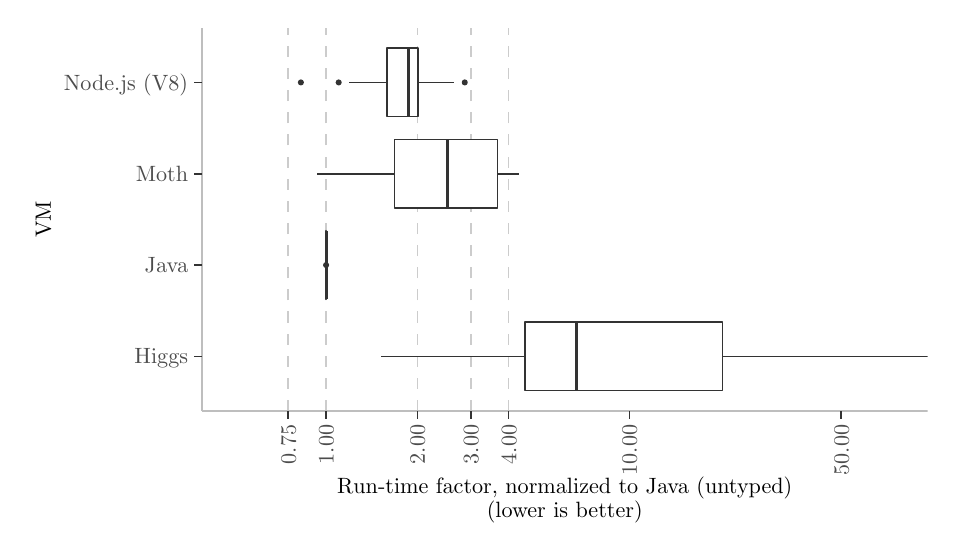
\begin{tikzpicture}[x=1pt,y=1pt]
\definecolor{fillColor}{RGB}{255,255,255}
\path[use as bounding box,fill=fillColor,fill opacity=0.00] (0,0) rectangle (325.21,180.67);
\begin{scope}
\path[clip] ( 62.92, 42.11) rectangle (325.21,180.67);
\definecolor{drawColor}{gray}{0.80}

\path[draw=drawColor,line width= 0.6pt,dash pattern=on 4pt off 4pt ,line join=round] ( 94.14, 42.11) -- ( 94.14,180.67);

\path[draw=drawColor,line width= 0.6pt,dash pattern=on 4pt off 4pt ,line join=round] (107.83, 42.11) -- (107.83,180.67);

\path[draw=drawColor,line width= 0.6pt,dash pattern=on 4pt off 4pt ,line join=round] (140.82, 42.11) -- (140.82,180.67);

\path[draw=drawColor,line width= 0.6pt,dash pattern=on 4pt off 4pt ,line join=round] (160.11, 42.11) -- (160.11,180.67);

\path[draw=drawColor,line width= 0.6pt,dash pattern=on 4pt off 4pt ,line join=round] (173.80, 42.11) -- (173.80,180.67);
\definecolor{drawColor}{gray}{0.20}

\path[draw=drawColor,line width= 0.6pt,line join=round] (251.09, 61.90) -- (325.21, 61.90);

\path[draw=drawColor,line width= 0.6pt,line join=round] (179.71, 61.90) -- (127.70, 61.90);
\definecolor{fillColor}{RGB}{255,255,255}

\path[draw=drawColor,line width= 0.6pt,line join=round,line cap=round,fill=fillColor] (251.09, 49.53) --
	(179.71, 49.53) --
	(179.71, 74.27) --
	(251.09, 74.27) --
	(251.09, 49.53) --
	cycle;

\path[draw=drawColor,line width= 1.1pt,line join=round] (198.42, 49.53) -- (198.42, 74.27);
\definecolor{fillColor}{gray}{0.20}

\path[draw=drawColor,line width= 0.4pt,line join=round,line cap=round,fill=fillColor] (107.83, 94.89) circle (  0.89);

\path[draw=drawColor,line width= 0.6pt,line join=round] (107.83, 94.89) -- (107.83, 94.89);

\path[draw=drawColor,line width= 0.6pt,line join=round] (107.83, 94.89) -- (107.83, 94.89);
\definecolor{fillColor}{RGB}{255,255,255}

\path[draw=drawColor,line width= 0.6pt,line join=round,line cap=round,fill=fillColor] (107.83, 82.52) --
	(107.83, 82.52) --
	(107.83,107.27) --
	(107.83,107.27) --
	(107.83, 82.52) --
	cycle;

\path[draw=drawColor,line width= 1.1pt,line join=round] (107.83, 82.52) -- (107.83,107.27);

\path[draw=drawColor,line width= 0.6pt,line join=round] (169.72,127.89) -- (177.61,127.89);

\path[draw=drawColor,line width= 0.6pt,line join=round] (132.50,127.89) -- (104.61,127.89);

\path[draw=drawColor,line width= 0.6pt,line join=round,line cap=round,fill=fillColor] (169.72,115.51) --
	(132.50,115.51) --
	(132.50,140.26) --
	(169.72,140.26) --
	(169.72,115.51) --
	cycle;

\path[draw=drawColor,line width= 1.1pt,line join=round] (151.54,115.51) -- (151.54,140.26);
\definecolor{fillColor}{gray}{0.20}

\path[draw=drawColor,line width= 0.4pt,line join=round,line cap=round,fill=fillColor] (157.94,160.88) circle (  0.89);

\path[draw=drawColor,line width= 0.4pt,line join=round,line cap=round,fill=fillColor] (112.38,160.88) circle (  0.89);

\path[draw=drawColor,line width= 0.4pt,line join=round,line cap=round,fill=fillColor] ( 98.72,160.88) circle (  0.89);

\path[draw=drawColor,line width= 0.6pt,line join=round] (141.06,160.88) -- (154.23,160.88);

\path[draw=drawColor,line width= 0.6pt,line join=round] (129.86,160.88) -- (115.96,160.88);
\definecolor{fillColor}{RGB}{255,255,255}

\path[draw=drawColor,line width= 0.6pt,line join=round,line cap=round,fill=fillColor] (141.06,148.51) --
	(129.86,148.51) --
	(129.86,173.25) --
	(141.06,173.25) --
	(141.06,148.51) --
	cycle;

\path[draw=drawColor,line width= 1.1pt,line join=round] (137.61,148.51) -- (137.61,173.25);
\end{scope}
\begin{scope}
\path[clip] (  0.00,  0.00) rectangle (325.21,180.67);
\definecolor{drawColor}{RGB}{190,190,190}

\path[draw=drawColor,line width= 0.6pt,line join=round] ( 62.92, 42.11) --
	( 62.92,180.67);
\end{scope}
\begin{scope}
\path[clip] (  0.00,  0.00) rectangle (325.21,180.67);
\definecolor{drawColor}{gray}{0.30}

\node[text=drawColor,anchor=base east,inner sep=0pt, outer sep=0pt, scale=  0.80] at ( 57.97, 59.15) {Higgs};

\node[text=drawColor,anchor=base east,inner sep=0pt, outer sep=0pt, scale=  0.80] at ( 57.97, 92.14) {Java};

\node[text=drawColor,anchor=base east,inner sep=0pt, outer sep=0pt, scale=  0.80] at ( 57.97,125.13) {Moth};

\node[text=drawColor,anchor=base east,inner sep=0pt, outer sep=0pt, scale=  0.80] at ( 57.97,158.12) {Node.js (V8)};
\end{scope}
\begin{scope}
\path[clip] (  0.00,  0.00) rectangle (325.21,180.67);
\definecolor{drawColor}{gray}{0.20}

\path[draw=drawColor,line width= 0.6pt,line join=round] ( 60.17, 61.90) --
	( 62.92, 61.90);

\path[draw=drawColor,line width= 0.6pt,line join=round] ( 60.17, 94.89) --
	( 62.92, 94.89);

\path[draw=drawColor,line width= 0.6pt,line join=round] ( 60.17,127.89) --
	( 62.92,127.89);

\path[draw=drawColor,line width= 0.6pt,line join=round] ( 60.17,160.88) --
	( 62.92,160.88);
\end{scope}
\begin{scope}
\path[clip] (  0.00,  0.00) rectangle (325.21,180.67);
\definecolor{drawColor}{RGB}{190,190,190}

\path[draw=drawColor,line width= 0.6pt,line join=round] ( 62.92, 42.11) --
	(325.21, 42.11);
\end{scope}
\begin{scope}
\path[clip] (  0.00,  0.00) rectangle (325.21,180.67);
\definecolor{drawColor}{gray}{0.20}

\path[draw=drawColor,line width= 0.6pt,line join=round] ( 94.14, 39.36) --
	( 94.14, 42.11);

\path[draw=drawColor,line width= 0.6pt,line join=round] (107.83, 39.36) --
	(107.83, 42.11);

\path[draw=drawColor,line width= 0.6pt,line join=round] (140.82, 39.36) --
	(140.82, 42.11);

\path[draw=drawColor,line width= 0.6pt,line join=round] (160.11, 39.36) --
	(160.11, 42.11);

\path[draw=drawColor,line width= 0.6pt,line join=round] (173.80, 39.36) --
	(173.80, 42.11);

\path[draw=drawColor,line width= 0.6pt,line join=round] (217.41, 39.36) --
	(217.41, 42.11);

\path[draw=drawColor,line width= 0.6pt,line join=round] (294.00, 39.36) --
	(294.00, 42.11);
\end{scope}
\begin{scope}
\path[clip] (  0.00,  0.00) rectangle (325.21,180.67);
\definecolor{drawColor}{gray}{0.30}

\node[text=drawColor,rotate= 90.00,anchor=base east,inner sep=0pt, outer sep=0pt, scale=  0.80] at ( 96.89, 37.16) {0.75};

\node[text=drawColor,rotate= 90.00,anchor=base east,inner sep=0pt, outer sep=0pt, scale=  0.80] at (110.58, 37.16) {1.00};

\node[text=drawColor,rotate= 90.00,anchor=base east,inner sep=0pt, outer sep=0pt, scale=  0.80] at (143.57, 37.16) {2.00};

\node[text=drawColor,rotate= 90.00,anchor=base east,inner sep=0pt, outer sep=0pt, scale=  0.80] at (162.87, 37.16) {3.00};

\node[text=drawColor,rotate= 90.00,anchor=base east,inner sep=0pt, outer sep=0pt, scale=  0.80] at (176.56, 37.16) {4.00};

\node[text=drawColor,rotate= 90.00,anchor=base east,inner sep=0pt, outer sep=0pt, scale=  0.80] at (220.16, 37.16) {10.00};

\node[text=drawColor,rotate= 90.00,anchor=base east,inner sep=0pt, outer sep=0pt, scale=  0.80] at (296.75, 37.16) {50.00};
\end{scope}
\begin{scope}
\path[clip] (  0.00,  0.00) rectangle (325.21,180.67);
\definecolor{drawColor}{RGB}{0,0,0}

\node[text=drawColor,anchor=base,inner sep=0pt, outer sep=0pt, scale=  0.80] at (194.07, 12.46) {Run-time factor, normalized to Java (untyped)};

\node[text=drawColor,anchor=base,inner sep=0pt, outer sep=0pt, scale=  0.80] at (194.07,  3.82) {(lower is better)};
\end{scope}
\begin{scope}
\path[clip] (  0.00,  0.00) rectangle (325.21,180.67);
\definecolor{drawColor}{RGB}{0,0,0}

\node[text=drawColor,rotate= 90.00,anchor=base,inner sep=0pt, outer sep=0pt, scale=  0.80] at (  8.36,111.39) {VM};
\end{scope}
\end{tikzpicture}
